\documentclass[11pt, executivepaper]{article}
\usepackage[utf8]{inputenc}
\usepackage[T1]{fontenc}
\usepackage{natbib}
\usepackage{amsmath, amsthm, amssymb}
\usepackage{amsfonts}
\usepackage{MnSymbol}
\usepackage{mathtools}
\usepackage{xcolor}
\usepackage{graphicx}
\usepackage{enumitem}
\usepackage{geometry}
 \geometry{
 a4paper,
 total={155mm,237mm},
 left=28mm,
 top=32mm,
 }
\usepackage{hyperref}
\hypersetup{colorlinks= true, allcolors=blue}
\setcitestyle{aysep={}}

\newtheorem{prop}{Proposition}

\begin{document}


\title{\textbf{On the Common Logical Structure of Classical and Quantum Mechanics}}

\author{Gabriele Carcassi\thanks{Physics Department, University of Michigan, Ann Arbor, MI 48109. E-mail: carcassi@umich.edu} \and Christine A. Aidala\thanks{Physics Department, University of Michigan, Ann Arbor, MI 48109. E-mail: caidala@umich.edu} \and Andrea Oldofredi\thanks{Section de Philosophie, Universit\'e de Lausanne, Switzerland. E-mail: Andrea.Oldofredi@unil.ch}}


\maketitle

\begin{abstract}
\center Notes on classical and quantum logic
\vspace{4mm}

\noindent \emph{Keywords}: Quantum Mechanics; Quantum Logic; Classical Logic; 
\end{abstract}
\vspace{5mm}
\clearpage

\tableofcontents
\vspace{5mm}

\section{Introduction}

As soon as Quantum Mechanics (QM) achieved a definite and coherent mathematical formulation, several physicists and philosophers claimed that its formal structure does not conform to the laws of classical propositional calculus, a belief that is widespread still to this day (cf.\ \cite{Giuntini:2002}, \cite{DallaChiara:2004} and \cite{deRonde:2016}). From the thirties, in fact, various modifications of Classical Logic (CL) were advanced in order to faithfully represent the physical content of quantum theory. For instance, in 1931 the Polish philosopher Zygmunt Zawirski proposed to apply \L ukasiewicz's three-valued logic to QM, starting from considerations about the wave-particle duality and Heisenberg's uncertainty principle. In virtue of the latter, moreover, the logical empiricists Moritz Schlick and Philipp Frank claimed that the conjunction of two or more statements may have no meaning in quantum theory, concluding that the classical conjunction is not always valid in the context of quantum physics, as recalled in \cite{Carnap:1966}. In their view, a typical example of invalid conjunction is one attributing a definite value for both position and momentum to a single quantum particle at a given time $t$. Furthermore, in 1933 Fritz Zwicky suggested that QM rejects the law of excluded-middle.\footnote{For historical details on quantum logic see \cite{Jammer:1974}.} However, it s generally recognized that 
the founding text on Quantum Logic (QL) is Birkhoff and von Neumann's essay ``\emph{The Logic of Quantum Mechanics}'' (\cite{vonNeumann:1936}), where the authors provided the standard account of the propositional calculus obeyed by quantum propositions.\footnote{It is worth noting that in his treatise \emph{Mathematische Grundlagen der Quantenmechanik} published in 1932 von Neumann had already stated that from the algebraic structure of quantum theory it is possible to formulate a new propositional calculus, anticipating seminal ideas that would have been fully expressed of his successive work in collaboration with Garrett Birkhoff.}

A few years after the publication of this paper, the research in quantum logic had a notable development in both the scientific and philosophical communities, opening new research programs searching for the correct formal structures to represent the physics of QM (cf.\ \cite{Reichenbach:1944}, \cite{Mackey:1957}, \cite{Finkelstein:1963}, \cite{Kochen:1965}, \cite{Jauch:1969}, \cite{Giuntini:2002}, \cite{DallaChiara:2004}), and intense metaphysical debates regarding the nature of logic itself and its empirical status (cf.\ notably \cite{Quine:1951}, \cite{Putnam:1968}, \cite{Dummett:1976}, \cite{Hallett:1982}, \cite{Weingartner:2004}, \cite{Bacciagaluppi:2009}). In addition, it is worth noting that research in quantum logic is still very prolific to the present day with many interesting applications in the fields of quantum information, computation and cryptography. Therefore, although QL is no longer viewed as a solution to the foundational problems affecting quantum theory\footnote{This conclusion is now widespread among experts as exemplified e.g.\ by \cite{Bacciagaluppi:2009} and \cite{Giuntini:2002}. Referring to this, the latter authors stated explicitly that ``quantum logics are not to be regarded as a kind of ``clue'', capable of solving the main physical and epistemological difficulties of QT [quantum theory]. This was perhaps an illusion of some pioneering workers in quantum logic'' (\cite{Giuntini:2002}, p.\ 225).}, it is an important discipline of contemporary physics. In this paper we will neither take a stance in the dispute concerning the ontological status of logic and its laws, nor we will consider recent developments of QL given that they are not strictly relevant to the point we are going to make. Indeed, the present essay is focused on the logical structures common to both quantum and Classical Mechanics (CM), following the spirit of the former discussion.\footnote{In the present essay we will be concerned only with propositional calculus in the context of non-relativistic QM. First order and higher order logics will not be discussed here as well as the logic of relativistic quantum theories.} 

Recently one of us asked in another essay whether quantum physics necessarily implies a revision of classical logic (cf.\ \cite{Oldofredi:2020}). Alternatively stated, it was asked whether classical logic must be abandoned in the quantum realm or there are quantum theories compatible with a classical propositional calculus. Analyzing Bohmian Mechanics, a well-known interpretation of QM, it has been showed that quantum physics does not necessarily involves a departure from classical logic. More precisely, it has been argued that in the context of BM not only the logical connectives retain their classical meanings---in particular the negation and the disjunction do follow CL---but also the distributivity law holds, contrary to the case of standard QM. This fact is a consequence of the clear ontology of the theory and its its theory of measurement.

In this paper we will be concerned with a similar issue, since we ask whether standard quantum mechanics necessarily involves a new logical structure radically different with respect to classical propositional calculus. In what follows we will answer this question in the negative. More precisely, here we have a three-fold aim: in the first place, we will analyze the main motivations and justifications for the introduction of quantum logic, arguing that they do not entail the failure of CL in the quantum context. In the second place we argue that classical and quantum mechanics share a common algebraic structure which can originate a classical propositional calculus for quantum propositions. A position dissimilar to the received view about QL. Here we will also show that several important statements in quantum mechanics, i.e.\ those concerned with expectation values, are not captured by QL, while they may be taken into account in a classical logical system. Finally, we will argue that it is possible to show that classical propositions may obey a quantum logic. Clearly, we will also spell out the reasons for which CL seems not to work in the context of QM. All these aspects, to our knowledge, are not sufficiently discussed in literature, thus, the present paper can contribute to shed new light on the relation between logic and quantum mechanics.
\vspace{2mm}

The essay is structured as follows: Section \ref{QL} provides a brief outline of the standard approach to QL (readers familiar with Birkhoff and von Neumann's proposal can skip this part), while in Section \ref{Motivations} we review the main motivations that have been given in literature to introduce a quantum logical calculus, explaining also why they do not entail the failure of classical logic in QM. In Section \ref{Math} we provide a mathematical argument aimed at showing not only that QM is compatible with classical logic---sharing a common logical structure with classical mechanics---but also that important sentences of quantum theory are excluded by standard QL, as stated a few lines above.\ In Section \ref{Discussion} we discuss the main philosophical implications of the preceding sections, and Section \ref{conc} concludes the paper.


\section{The Standard Approach to Quantum Logic}
\label{QL}

In order to present the standard approach to QL, let us say a few words about the relation between classical logic and classical mechanics. It is a well known fact that classical propositional logic is equivalent to a Boolean algebra where propositions (atomic and complex) have truth values ``true'' and ``false'' (or 1 and 0), and the main operations among them are conjunction ``$\wedge$'', disjunction ``$\vee$'' and negation ``$\neg$'', the only unary operation. From these logical connectives one can introduce secondary operations, as for instance the material implication ``$\longrightarrow$'', the exclusive or ``$\oplus$'' and logical equivalence ``$\longleftrightarrow$''. Furthermore, it is important for our discussion to underline that the laws of propositional logic include commutativity, associativity, identity and distributivity with respect to $\wedge$ and $\vee$.

Analogously, the algebraic structure underlying classical mechanics is Boolean as well, being commutative, distributive and associative; in this context the logical operations of conjunction, disjunction and negation are replaced respectively by multiplication, addition and complementation among the variables of the theory. This fact has an interesting physical significance, since the variables associated to magnitudes of physical systems can be added and multiplied together---i.e.\ one can sum and multiply measurement results. Both propositional logic and classical mechanics, thus, generate a complemented Boolean lattice; from this fact it follows that the observable algebra of CM ``is isomorphic to a Boolean algebra of propositions with $(\wedge, \vee, \neg)$'' (\cite{David:2015}, p. 79).
To this regard, Beltrametti claims that 
\begin{quote}
Boolean algebras are algebraic models of classical logic (more specifically of classical propositional calculus) with the algebraic operations of meet ($\wedge$) and join ($\vee$) corresponding to the logical connectives ``and'', ``or'', and the unary relation of orthocomplementation corresponding to the logical negation. The rules and tautologies of classical logic have their counterpart in equations and identities of Boolean algebras (\cite{Beltrametti:2004}, p.\ 341). 
\end{quote}

Therefore, it is possible to formally characterize the state of a physical system via logical propositions which can assume the truth values ``true'' or ``false''---depending whether such statements describe true or false state of affairs concerning the system under consideration (cf.\ \cite{Jaeger:2009}, p. 61)---and to perform logical operations among propositions via the connectives $(\wedge, \vee, \neg)$. It is worth noting that in the context of CM it is always determined whether a system instantiates a given property or not; alternatively stated, every logical proposition about physical systems is either true or false, and hence in CM the principle of semantic bivalence holds (for more details cf.\ \cite{Bub:2007}, p.\ 642, \cite{Giuntini:2002}, p.\ 130).
 
Taking instead into account the mathematical structure and the physical content of standard QM, it is generally claimed that the classical propositional calculus is no longer appropriate to represent the logic obeyed by quantum propositions, since quantum theory does not share the same algebraic structure of classical mechanics. In particular, the algebra of quantum observables is non-commutative and, from a logical perspective, generates a non-distributive orthocomplemented lattice, which is non-Boolean. 
Referring to this, given the axioms of QM Birkhoff and von Neumann showed how the physical content of the theory does not conform to a classical logical structure. The principal aim of their founding essay of quantum logic was to ``discover what logical structures one may hope to find in physical theories which, like quantum mechanics, do not conform to classical logic'' (\cite{vonNeumann:1936}, p.\ 823). The expression quantum logic in this paper must be clarified, since it refers to a quantum propositional calculus in the form of a ``calculus of linear subspaces with respect to \emph{set products}, \emph{linear sums}, and \emph{orthogonal complements}'' which ``resembles the usual calculus of propositions with respect to \emph{and}, \emph{or}, and \emph{not}'' (\emph{ibid}.), where the logical propositions are associated to measurements, tests on quantum systems.\footnote{Cf.\ \cite{Giuntini:2002} and \cite{DallaChiara:2004} for a systematic introduction to various forms of quantum logics, and to \cite{Engesser:2009} for historical and philosophical discussions on the topic.}

Their analysis begins by defining quantum logical propositions as \emph{experimental propositions}, i.e.\ statements affirming that a certain observable $A$ (or a set of observables) measured on a quantum system $s$ has a given value $a_i$ (or a sequence of values). More precisely, the authors stress that both in classical and quantum mechanics observations of physical systems are given by readings of experimental outcomes ($x_1, \dots, x_n$) of \emph{compatible} measurements ($\mu_1, \dots, \mu_n$). The values ($x_1, \dots, x_n$) are elements of what the authors called the ($x_1, \dots, x_n$)-space, i.e.\ the ``observation-space'' of the system in question, whose elements are all the possible combinations of results of the compatible measurements ($\mu_1, \dots, \mu_n$). Hence, the actual values ($x_1, \dots, x_n$) form a subset of such a space. Birkhoff and von Neumann, then, defined the experimental propositions concerning a physical system as the subsets of the observation space associated with it.

Secondly, the authors underlined that in classical and quantum mechanics the states of physical systems are mathematically represented by points in their state spaces---phase space for the classical case, and Hilbert space $\mathcal{H}$ for the quantum case---which provide the maximal information concerning the system. A point in phase space corresponds to the specification of the position and momentum variables of a certain classical system, whereas in QM the points of $\mathcal{H}$ correspond to wave functions. The authors, then, find a connection between subsets of the observation-space of a system and subsets of its Hilbert space, specifying that quantum experimental propositions are mathematically represented by a closed linear subspace of $\mathcal{H}$; this step is crucial in order to obtain the quantum propositional calculus.\ Alternatively, we can say that quantum mechanical operators correspond to propositions with ``yes/no'' (``true/false'') outcome in a logical system\footnote{Cf.\ also \cite{David:2015}, p.\ 78, where we read that ``An orthogonal projector $\textbf{P}$ onto a linear subspace $P\subset\mathcal{H}$ is indeed the operator associated to an observable that can take only the values 1 (and always 1 if the state $\psi\in P$ is in the subspace $P$) or 0 (and always 0 if the state $\psi\in P^{\perp}$ belongs to the orthogonal subspace to $P$).\ Thus we can consider that measuring the observable $\textbf{P}$ is equivalent to perform a test on the system, or to check the validity of a logical proposition $p$ on the system''.} as underlined by Svozi:
\begin{quote}
Any closed linear subspace of---or, equivalently, any projection operator on---a Hilbert space corresponds to an elementary
proposition. The elementary \emph{true--false} proposition can in English be spelled out explicitly as
\begin{quote}
``The physical system has a property corresponding to the associated closed linear subspace'' (\cite{Svozi:1999}, p.\ 1).
\end{quote}
\end{quote}

Thus, since in quantum mechanics physical systems do not have well-defined values for their properties before the measurement of a given operator (contrary to their classical counterparts), or better that quantum observations do not reveal pre-existing values, we have to stress that such quantum propositions refer always to measurements or to preparation procedures. Hence, the sentence ``the particle $s$ has $x$-spin up'' means either that I have measured the observable $S_x$ and I have found the value $+\hbar/2$ associated with the state ``$x$-spin-up'', or equivalently that I prepared $s$ in the $x$-spin-up state. Thus, one cannot simply say, as in classical mechanics, that a certain system has a certain property without having prepared such a system in a given state or having measured it.\footnote{More on this below.}

Now that we have clarified what quantum propositions are, let us introduce Birkhoff and von Neumann's quantum logic. In order to properly define a propositional calculus for QM, one must define the logical operators for conjunction, disjunction and negation and the notion of logical implication. Following \cite{vonNeumann:1936}, the procedure is rather simple: 
\begin{enumerate}
\item The negation of a proposition $p$ is defined by the authors as follows: ``since all operators of quantum mechanics are Hermitian, the mathematical representative of the negative of any experimental proposition is the orthogonal complement of the mathematical representative of the proposition itself'' (\cite{vonNeumann:1936}, pp.\ 826-827). The orthogonal complement $P^{\perp}$ of the subspace $P$ is the set whose elements are all the vectors orthogonal to the elements of $P$. Such an orthogonal complement satisfies the following property: given a subset $P\subset\mathcal{H}$ and a pure state $\psi$, $\psi(P)=1$ iff $\psi(P^{\perp})=0$ and $\psi(P)=0$ iff $\psi(P^{\perp})=1$. As Dalla Chiara and Giuntini underline, ``$\psi$ assigns to an event probability 1 (0, respectively) iff $\psi$ assigns to the orthocomplement of $P$ [notation adapted] probability 0 (1, respectively). As a consequence, one is dealing with an operation that \emph{inverts} the two extreme probability-values, which naturally correspond to the truth-values \emph{truth} and \emph{falsity} (similarly to the classical truth-table of negation)'' (\cite{Giuntini:2002}, p.\ 132).
\item Concerning the conjunction, Birkhoff and von Neumann notice that one can retain the very same set-theoretical interpretation of the classical conjunction in QL, since the intersection of two closed subspaces $P, Q\subset\mathcal{H}$ is still a closed subspace. Thus, one maintains the usual meaning for the conjunction: the pure state $\psi$ verifies $P\cap Q$ iff $\psi$ verifies both $P$ and $Q$. Thus, quantum logic does not introduce a new logical operator for the conjunction.
\item Contrary to the previous case, the logical operator for disjunction cannot be represented by the set-theoretic union, since the set-theoretical union of the two subspaces $P, Q$ will not be in general a subspace, thus, it is not an experimental proposition. Therefore, in QL one introduces the quantum logical disjunction as the the closed span of the subspaces $P, Q$, which is an experimental proposition. Such a statement corresponds to the ``smallest closed subspace containing both $P$ and $Q$'' (\cite{Bacciagaluppi:2009}, p.\ 55). 
\item The logical implication is defined by set theoretical inclusion: given two experimental propositions $p$ and $q$, 
$p$ implies $q$, means that whenever one predicts $p$ with certainty, one can predict also $q$ with certainty, and this is equivalent to state that $p$ is a subset of $q$. This fact is particularly important since the authors showed that ``it is \emph{algebraically} reasonable to try to correlate physical qualities with subsets of phase-space'' and thus, ``physical qualities attributable to any physical system form a partially ordered system'' (\cite{vonNeumann:1936}, p.\ 828, notation adapted).
\end{enumerate}

In this manner we have defined a propositional calculus for quantum experimental propositions, which generates an orthocomplemented lattice. In what follows we analyze the motivations for such a quantum logic, clarifying why it is generally believed that classical propositional calculus cannot be applied in QM. 

\section{Quantum Disjunction and Distributivity Law}
\label{Motivations}

The first remarkable difference between QL and CL is the failure of the distributive law. It is a well-known fact that such a law holds in the propositional calculus underlying classical mechanics in virtue of the commutative algebra of classical observables.
Referring to this, \cite{Giuntini:2002} claim that distributivity fails in quantum logic for two main reasons:
\begin{itemize}
\item the non-commutativity of quantum observables,
\item the peculiar behavior of the quantum disjunction---which may be true although neither of the member is true in virtue of the linearity of the Schr\"odinger Equation (SE)---the other major deviation from classical logic. 
\end{itemize}
\noindent Let us then have a closer look to these motivations for the failure of the distributivity law and more generally of CL in the quantum context.

Contrary to the case of classical mechanics, QM relies on a non-commutative algebraic structure\footnote{For details on the mathematical structure of QM and its physical content the reader may refer e.g.\ to \cite{Sakurai1994}, and \cite{Griffiths:2014}. In this essay, it is assumed that the reader has some familiarity with the standard formalism of QM.}: quantum observables generally do not commute, meaning that for any pair of operators $A,B$ we have $[A,B]=AB-BA\neq0$. From a physical perspective this fact entails that if one performs a measurement of $A$ on a quantum system followed by a measurement of $B$, in general one will obtain different results inverting the order of these observations. Moreover, in virtue of the non-commutative structure of quantum theory, to measure an operator $C=A+B$ is not typically equivalent to measure $A$ and $B$ independently and then add the respective results, since $A,B$ will be in general incompatible (cf.\ \cite{David:2015}, p.\ 77). This algebraic fact of QM constitutes the formal basis to prove the Heisenberg uncertainty relation, a theorem of quantum theory which reflects the operational inability to simultaneously measure the values of incompatible operators with arbitrary precision. Such a result, in turn, is usually interpreted ontologically in the sense that quantum system do not instantiate definite properties in non-measurement situations (cf.\ \cite{Sakurai1994}).

In addition, as we will explain in the remainder of this section, the failure of distributivity in quantum logic is due to another particular feature of this new propositional calculus, namely on the behavior of the quantum disjunction, which is due to the presence of quantum superpositions. Indeed, another remarkable difference between QM  and CM is that quantum systems can be in superposition states as a consequence of the linearity of the Schr\"odinger equation---the fundamental dynamical law of QM---which for a single particle reads: 
\begin{align}
\label{SE}
i\hbar\frac{\partial\psi}{\partial t}=\Big(-\frac{\hbar^2}{2m}\nabla_k^2+V\Big)\psi=H\psi,
\end{align}
\noindent where $H$ represents the Hamiltonian operator, defined as the sum of kinetic and potential energy of the system at hand. More specifically, this algebraic property of \eqref{SE} entails that if two wave functions\footnote{In QM the wave function of a system provides the maximal information available about it.} $\psi_1, \psi_2$ are both possible solutions of the same Sch\"odinger equation, then their linear combination (\emph{superposition}) 
\begin{align}
\label{SSE}
\psi_s=\alpha\psi_{1}+\beta\psi_{2}
\end{align} 
is still a solution of the same SE---$|\alpha|^2,|\beta|^2$ (with $\alpha,\beta\in\mathbb{C}$) represent the probabilities to find the system in $\psi_1, \psi_2$ respectively. Notably, the new superposed state $\psi_s$ is also a consistent representation of the system. Referring to this,  \cite{deRonde:2016} explicitly say that in QL ``differently from the case in classical semantics, a quantum disjunction may be true even if neither of it members is true. This reflects, for example, the case in which we are dealing with a state such as that of a spin $1/2$ system which is in a linear combination of states up and down'', as in the example we are going to consider in order to explain the failure of distributivity in the quantum context. 

To claim that in quantum logic conjunction and disjunction are not distributive means that given three propositions $p, q$ and $r$ the logical law
\begin{align}
\label{DL}
p\wedge(q\vee r)\longleftrightarrow(p\wedge q)\vee(p\wedge r)
\end{align}

\noindent does not hold.\footnote{In the context of quantum logic, distributivity must be replaced by a weaker law: $(p\wedge q)\vee(p\wedge r)\longrightarrow(p\wedge(q\vee r)).$}
Let us explain this fact with a simple example taken from \cite{Giuntini:2002}. Suppose to consider a $1/2-$spin particle, let's say an electron and assume that this paritlce has spin up along the $x$ axis. From QM we know that there are only two possible spin states in which a particle can be found in each axis after a spin measurement, namely either in the up or in the down state. Furthermore, since spin operators along different axis do not commute, being incompatible observables---$[S_x, S_y]=[S_x, S_z]=[S_y, S_z]\neq0$---they cannot be simultaneously measured. Then, as a consequence of the Heisenberg uncertainty principle, ``both propositions ``$spin_y$ is up'' and ``$spin_y$ is down'' shall be strongly undetermined. However, the disjunction ``either $spin_y$ is up or $spin_y$ is down'' must be true'' (\cite{Giuntini:2002}, pp.\ 133-134), and the same holds for the case of spin in the $z$ direction. Therefore, if $p$ in \eqref{DL} represents the proposition ``the electron has $x$-spin up'', $q$ the proposition ``the electron has $y$-spin up'' and $r$  the proposition `the electron has $y$-spin down'', it is possible to see that the first part of \eqref{DL} express a true statement---i.e.\ $p\wedge(q\vee r)=1$---whereas $(p\wedge q)$ and $(p\wedge r)$ are both false in virtue of the incompatibility between the spin operators among different axes, implying that the second part of the distributive law asserts a false statement, i.e.\ $(p\wedge q)\vee(p\wedge r)=0$. Consequently, this law fails in the context of quantum theory, since we have $p\wedge(q\vee r)=1\longleftrightarrow(p\wedge q)\vee(p\wedge r)=0$. 
\vspace{2mm}

In what follows we will stress that these motivations for QL are not sufficient to claim that CL is rejected by quantum theory.

\subsection{Disjunction}

Connection between disjunction and superposition.

``A relevant feature of $\vee$ is that, differently from the case in classical semantics, a quantum disjunction may be true even if neither of it members is true. This reflects, for example, the case in which we are dealing with a state such as that of a spin 1/2 system which is in a linear combination of states up and down. Both propositions, ``the state is up'' and ``the state is down,'' may have no definite truth value (the excluded middle principle is violated), but the disjunction ``the state is up or the state is down'' is a tautology.''

\begin{description}
	\item $p =$ ``The particle has spin $z^+$''
	\item $q =$ ``The particle has spin $z^-$''
\end{description}

Claim: $p \vee q$ is \textbf{always} true, even if $p$ and $q$ may possibly be both false. The idea is that $p \vee q$ includes also all superpositions of $p$ and $q$.

Counterclaim. The propositions $p$ and $q$ are experimentally equivalent to:
\begin{description}
	\item $p =$ ``The expectation value for $S_z$ is 1/2$\hbar$''
	\item $q =$ ``The expectation value for $S_z$ is -1/2$\hbar$''
\end{description}
The proposition $p \vee q$ corresponds to the statement ``The absolute value of the expectation value for $S_z$ 1/2$\hbar$''. If we have a superposition of $p$ and $q$, the expectation value for $S_z$ will be strictly between $-1/2 \hbar$ and $1/2 \hbar$, and therefore $p \vee q$, when discussing expectation values, will be false as one would expect.

\subsection{Distributivity}

The distributivity in quantum mechanics is ``weird'' because (1) it can be true even if none of the elements of the disjunction is true due to the linearity of the Schr\"ondinger equation and (2) quantum observables do not commute. 

\begin{description}
    \item $p =$ ``The particle has spin $x^+$''
    \item $q =$ ``The particle has spin $y^+$''
    \item $r =$ ``The particle has spin $y^-$''
\end{description}

Classic: $p \wedge (q \vee r)$ if and only if $(p \wedge  q) \vee (p \wedge r)$

Quantum: Assume $p$ is true, which means we measured spin $x$ to be $+$. Since if I measured spin $y$ I would either get $+$ or $-$, we have $q \vee r \equiv \top$. Therefore $p \wedge (q \vee r)$ is true. On the other hand, both terms in the second disjunctions are false: because $p \wedge  q$ refer to incompatible observables, we have $p \wedge  q \equiv \bot$. Therefore the $(p \wedge  q) \vee (p \wedge r) \equiv \bot$.

\subsubsection{Reframing}

2 casi: considerare

\begin{description}
    \item $p =$ ``The state of particle at time $t$ is $x^+$''
    \item $q =$ ``The state of particle at time $t$ is $y^+$''
    \item $r =$ ``The state of particle at time $t$ is $y^-$''
\end{description}

Then all three assertions are incompatible with each other. That is, $p \wedge q \equiv q \wedge r \equiv r \wedge p \equiv \bot$. Therefore $p \wedge (q \vee r) \equiv \bot \equiv (p \wedge  q) \vee (p \wedge r)$.

\begin{description}
    \item $p =$ ``The state of particle at time $t$ is $x^+$''
    \item $q =$ ``The state of particle at time $t$ is $y^+$''
    \item $r =$ ``The state of particle at time $t$ is $y^-$''
    \item $\hat{q} =$ ``The state of particle at time $\hat{t}$ is $y^+$''
    \item $\hat{r} =$ ``The state of particle at time $\hat{t}$ is $y^-$''
\end{description}

In this case $p \wedge \hat{q} \not\equiv \bot$ and $p \wedge \hat{r} \not\equiv \bot$. Therefore the original claim was $p \wedge (\hat{q} \vee \hat{r})$ if and only if $(p \wedge  q) \vee (p \wedge r)$ which is not the classical logic distributive law. Note that, $\hat{q} \vee \hat{r} \equiv \top$ under condition that ``We measure spin $y$ at time $\hat{t}$''.

\subsubsection{Classical example}
\begin{center}
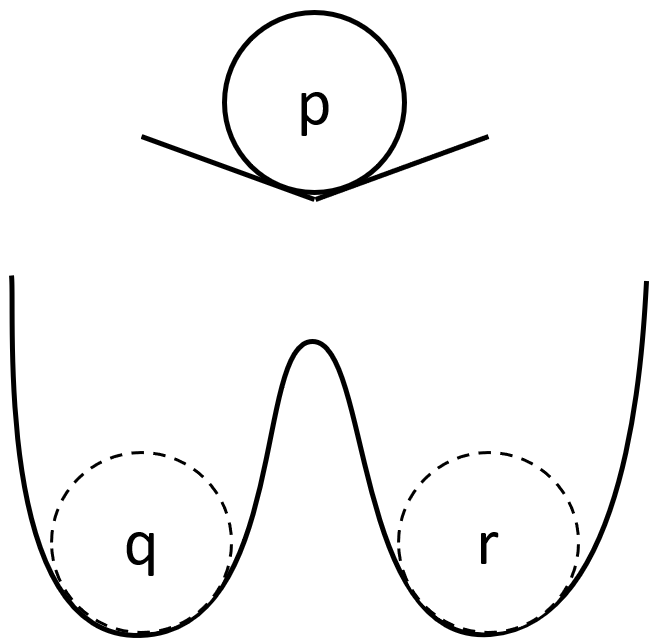
\includegraphics[scale=.3]{Balldrop.png}
\end{center}

We have a ball sitting at position $p$ over a hatch. If the hatch opens, the ball drops, bounces around, until it will rest at either position $q$ or $r$ with equal chance. Two cases, as before:

\begin{description}
    \item $p =$ ``The position of the ball at time $t$ is $p$''
    \item $q =$ ``The position of the ball at time $t$ is $q$''
    \item $r =$ ``The position of the ball at time $t$ is $r$''
\end{description}

These are three incompatible assertions. Distributivity holds as before.

\begin{description}
    \item $p =$ ``The position of the ball at time $t$ is $p$''
    \item $q =$ ``The position of the ball at time $t$ is $q$''
    \item $r =$ ``The position of the ball at time $t$ is $r$''
    \item $\hat{q} =$ ``The position of the ball at time $\hat{t}$ is $q$''
    \item $\hat{r} =$ ``The position of the ball at time $\hat{t}$ is $r$''
\end{description}

We assume that, after time $t$, the hatch is opened and that at time $\hat{t}$ the ball has settled. As before, $\hat{q} \vee \hat{r} \equiv \top$ because the ball must be in one of the two positions after it dropped, therefore, if $p$ is true, the left side of the biconditional is true while the right side is false.

%\section{Classical and quantum parallel}
%
%Classical state: $\rho(x,p)$
%
%Quantum state: $\psi(x)$
%
%Classical observable $f(x,p)$. Average value $<f> = \int f(x, p) \rho(x, p) dx dp$. Eigenstate $f(x, p) \rho(x, p) = f_0 \rho(x, p)$.
%
%Quantum observable $F$. Average value $<F> = \int \psi^\dagger(x) F \psi(x) dx$. Eigenstate $F \psi(x) = f_0 \psi(x)$.
%
%In both cases, average value equal to $f_0$ means that the contributions of all parts of the ensemble combine to the value $f_0$. Eigenstate $f_0$ means all parts of the ensemble contribute the same value $f_0$.
%
%For example, a classical eigenstate of $H = \frac{p^2}{2m} + \frac{1}{2} k x^2$ with eigenvalue $e_0$ is any function $\rho(x,p)$ that is different from zero only on the ellipses with energy $e_0$. That is, all elements of the distribution have the same energy.
%
%The statement ``the observable $f$ of the system is between $f_0$ and $f_1$'' is therefore unclear. It could be taken to mean ``the average of observable $f$ of the system is between $f_0$ and $f_1$'' or ``the observable $f$ for each part of the ensemble is between $f_0$ and $f_1$''. In the first case, we are identifying a value from the real line, using the standard topology and the standard Borel algebra. In the second case, we are identifying a set of possible functions based on their support.
%
%Now suppose that the $U$ and $V$ are two intervals. We have ``the average $<f>$ is in $U \cup V$'' is  equivalent to ``the average $<f>$ is in $U$'' $\vee$ ``the average $<f>$ is in $V$''. The average value must be in and and only one set. We also have ``the support of $\rho$ is $U \cup V$'' is not equivalent to ``the support of $\rho$ is $U$'' $\vee$ ``the support of $\rho$ is $V$''. The dis tribution could span both sets at the same time. But the lattice generated by such sets is still a $\sigma$-algebra, and therefore follows classical logic.
%
%To check/prove: neither algebras is a sub-algebra of the other; both sub-algebras of the norm-induced one.

\section{Math}
\label{Math}

In this section we present our main argument, which is that the state space of quantum mechanics and the space of classical probability distributions possess a similar structure that allows one to apply distributive propositional calculus (i.e. ``classical logic'') on the first and non-distributive propositional calculus (i.e. ``quantum logic'') on the second. That is, both theories will have two lattices of propositions: a distributive one that follows classical logic and a non-distributive one that follows quantum logic.

Note that the classical space we will be using is not phase-space itself, but the space of probability distributions over phase-space, which is a real Hilbert space and thus has a similar structure to the quantum counterpart. The central point is that many features of quantum logic stem not from quantum mechanics per-se, but from the fact that quantum mechanics is a probabilistic theory, which means a classical probabilistic theory will share the same features. We find that the main point of confusion stems from comparing quantum theory, which is inherently a probabilistic theory, to a non-probabilistic classical theory. This approach does not allow one to understand which differences are due to the classical/quantum nature of the theory, and which are due simply to the probabilistic/non-probabilistic nature. By comparing quantum theory to a probabilistic classical theory, we put ourselves in a position to fully understand which difference is due to what, and have a much clearer understanding of both.\footnote{Note that probabilistic theories are important even in classical mechanics. Due to the nature of experimental verification, even in classical mechanics, there are always going to be uncertainties in the preparation and measurements, and repeated measurements will always lead to statistical constructs.} Critically, we will see that the non-distributivity of the quantum logic lattice does not originate from non-commuting observables or superposition of quantum mechanics: it is a property of the lattice of subspaces of any vector space and, indeed, of the lattice of sugroups of any group more in general. [CITE: Introduction to Lattices and Order Theory, Davey, Priestley - 2002 CUP]

Mathematically, the distributive lattice will be provided in both classical and quantum mechanics by the Borel algebra, the smallest $\sigma$-algebra that contains the topology; the non-distributive lattice will be provided by the set of subgroups ordered by inclusion. We will see that the non-distributive lattice is a strict subset of the distributive one, meaning that everything that can be described in quantum logic can also be described in classical logic. Moreover, the distributive lattice will include propositions, like propositions on the expectation value of observables, that are of scientific interest.\footnote{In an experimental context, in fact, by ``measurement'' one typically refers to the statistical collection of many ``single takes''. Quantum logic describes the single-take measurements. For example, measurements of cross sections, the most typical type of measurement in the context of particle physics, are not part of the quantum lattice, and neither are measurements of the probabilities themselves.}

%they do not seem well-known among physicists and philosophers of science, therefore we briefly summarize their definition, use and meaning. [CITE: Kelly, Logic of Reliable Inquiry - Carcassi/Aidala, Assumptions of Physics]

%It is useful, at this point, to review $\sigma$-algebras, which are foundational structures in mathematics,

Note that mathematical branches important in the context of physics, like measure theory [CITE: Measure theory, by Donald L. Cohn] and probability theory,[CITE: Grimmet/Stirzaker, Probability and Random Processes] are built not top of $\sigma$-algebras, which should be considered foundational structure. Let us therefore review some crucial aspects.

We start with a set $X$. In the quantum case, this will correspond to the set of all possible quantum states. In the classical case, this will corrsepond to the set of all possible probability distributions over phase space. We should stress, however, that $\sigma$-algebras are defined independently of what the elements of $X$ actually are. For a simpler example, $X$  could correspond to the set of the real numbers for a continuous quantity. A $\sigma$-algebras is a collection of subsets of $X$, closed under countable union, countable interesection and complement with respect to $X$, meaning that performing those operations on the sets contained in a $\sigma$-algebra will return another set in the same $\sigma$-algebra. For example, a standard $\sigma$-algebras for the real numbers will typically contain all the open intervals $(a, b)$.

A collection of subsets may seem quite an abstract concept, but it can be readily made concrete: any statement on the objects represented by $X$ can be represented by a set. For example, the open set $(a, b)$ will exactly correspond to the statement ``the value of the quantity is between $a$ and $b$''. It is therefore useful to think about $\sigma$-algebras as collections of statements about $X$ instead of sets. As the $\sigma$-algebra is closed under countable union, countable intersection and complement with respect to $X$, the corresponding statements will be closed under countable conjunction, countable disjunction and complement: the $\sigma$-algebra can be thought as a Boolean algebra of statements. Note that this interpretation is exactly the one used in probability. In fact, a probability space is defined by three things: a sample space $\Omega$ which represents the set of all possible outcomes; a $\sigma$-algebra over $\Omega$ which represents all events, all propositions; and a measure that assigns a probability to each event.

Every topological space comes already equipped with a $\sigma$-algebra called Borel algebra. A topology, in fact, is also a collections of sets, called open sets, and the Borel algebra is defined to be the smallest $\sigma$-algebra that contains all the open sets. The topology will not be directly important for us, but only as a mean to construct the Borel algebra. Complete normed spaces, such as Hilbert spaces, have a canonical way to construct a topology and therefore a $\sigma$-algebra. Let us see first how it works in a standard three-dimensional Euclidean space. Given two points $x$ and $y$, we can write the square of distance $\epsilon^2 = |y - x|^2$ as the square of the norm of the vector between the two points. The statement ``the position is within $\epsilon$ meters of $x$'' corresponds to the set $U = \{y \; | \; |y - x|^2 < \epsilon^2 \}$ of all the points whose distance from $x$ is less than $\epsilon$. These are exactly the open sets that generate the topology, and the Borel algebra will be the smallest $\sigma$-algebra that contains these sets. This works in the same way for all normed spaces. A Hilbert space, in particular, comes with an inner product which also defines a norm. We can define a distance $\epsilon^2 = |\psi - \phi|^2=\langle \psi - \phi , \psi - \phi \rangle$ between two states, and the statement ``the state of the system is within $\epsilon$ of $\psi$'' corresponds to the set $U = \{\phi \; | \; |\psi - \phi|^2 < \epsilon^2\}$. As we'll see later, the space of classical probability distributions is also a Hilbert space where each point corresponds to the square root of the density.\footnote{The choice of the square root of the density over the density itself is really a technical choice. Of all the $L^p$ spaces, the only Hilbert space is $L^2$, the space of the square-integrable functions.} We will have a distance $\epsilon^2 = |\sqrt{\rho_1} - \sqrt{\rho_2}|^2=\langle \sqrt{\rho_1} - \sqrt{\rho_2} , \sqrt{\rho_1} - \sqrt{\rho_2} \rangle$ and we can proceed in the same exact way. In all normed spaces, the topology is constructed from sets of the form ``the object is within $\epsilon$ of $x$''.\footnote{In the case of Hilbert spaces and quantum mechanics, the map between topology and experimental verification does not work perfectly because absolute modulus and phase are not physically meaningful. This can be fixed by using the corresponding projective space, which removes the overdetermination. We are not going to do this as projective spaces have their own peculiarities and are used less.}


It is a simple result that the Borel algebra thus constructed contains all propositions of quantum logic.

\begin{prop}
	Let $H$ be a Hilbert space. Let $\Sigma$ be the Borel $\sigma$-algebra induced by its inner product. Let $L(H)$ be the lattice of closed subspaces of $H$. Then $L(H) \subset \Sigma$.
\end{prop}

Proof. Let $p \in L(H)$ be a closed sub-space of $H$. Then $p$ is a closed set, the complement of an open set, and therefore a Borel sets: $p \in \Sigma$. Let $v \in H$ be a vector in the Hilbert space and consider the singleton $U = \{ v \}$. This is not a closed sub-space and therefore $U \notin L(H)$. As the topology of a Hilbert space is Hausdorff, all singletons are closed and therefore $U \in \Sigma$. This means $L(H) \subset \Sigma$. This concludes the proof.

In quantum logic, the propositions corresponded to closed subspaces, which are closed sets and are therefore Borel sets. All the propositions of quantum logic are therefore readily found in the Borel algebra of the Hilbert space. The Borel algebra, which is a Boolean algebra that follows classical logic, contains also all the statements of quantum logic. This construction also applies identically for the classical cases, where we will also be able to talk about the set of all closed subspaces which will have a parallel structure.

While all of this may seem daunting to someone who has never seen this material, we want to stress that these are very standard constructions. We are not taking some obscure framework from some fringe field of mathematics: these are the standard mathematical techniques used to study these spaces and can be found in any textbook. [CITE: Elements of Hilbert Spaces and Operator Theory, Harkrishan Lal Vasudeva, https://www.springer.com/gp/book/9789811030192 ] What we are doing here is bringing out their full physical significance, which is too often overlooked. Understanding the link between the mathematical structures and the physics they represent is crucial to clearing out possible misunderstandings.

Now that we have briefly seen the definitions and basic constructions, we can gain more insights into these structures and what they represent. First, let us understand why the lattice of subspaces (i.e. quantum logic) fails to be a Boolean algebra. Stone's representation theorem tells us that any Boolean algebra can be expressed as an algebra of sets using the standard set operations (i.e. intersection, union and complement). For the lattice of subspaces, note that the disjunction $p \vee q$ does not correspond to the set union of the subspaces, but the span. In fact, the union of subspaces is not part of the lattice.  This is why the lattice, even if it is a complemented $0-1$ lattice, fails to be a Boolean algebra: it does not use the standard set operations.

Clearly, $\sigma$-algebras are Boolean algebras because they are exactly an algebra of sets with standard set operations. As we said before, the Borel algebra will contain the lattice of subspaces plus all the set operations between them, including the union. In a way, the lattice of subspaces is not Boolean because it does not contain enough sets, which are instead contained in the Borel algebra.

One may ask: do these extra sets correspond to physically meaningful propositions? To answer that, let us first demonstrate the following proposition.

\begin{prop}
	Let $H$ be a Hilbert space and $\langle \, , \, \rangle$ be its inner product. Let $X$ be a self-adjoint bounded linear operator. Let $F_X : H \to \mathbb{R}$ be the map defined by $F_X(\psi) = \langle \psi , X \psi \rangle$. Let $U \subseteq \mathbb{R}$ be a Borel set. Then $F_X^{-1}(U)$ is a Borel set.
\end{prop}

Proof. Let $X$ be a self-adjoint bounded linear operator. Recall that a linear operator is continuous if and only if it is bounded. Therefore $X$ is continuous. Note that $F_X$ is the composition of $X$ with the inner product. Recall that the inner product is a continuous function. Since $F_X$ is the composition of continuous functions it is also continuous. Recall that all continuous functions are also Borel measurable, therefore $F_X$ is Borel measurable. Let $U \subseteq \mathbb{R}$ be a Borel set. Since $F_X$ is Borel measurable, the reverse image $F_X^{-1}(U)$ is also a Borel set. This concludes the proof.

Since $\langle \psi , X \psi \rangle$ expresses the expected value for operator $X$, the proposition shows that the Borel algebra can express statements about the expectation value of observables,\footnote{Technically, position and momentum are not bounded operators. However, one can argue that measured position and momentum are indeed bounded as the acceptance of a detector is always limited. Note that all operators for which the spectral theorem applies can be written as the limit of a sequence of bounded operators.} such as ``the expected position $\langle x \rangle$ of the particle is between $x_0$ and $x_1$.'' This would correspond to the Borel set $\{ \psi \in H \, | \, \langle \psi , X \psi \rangle \in (x_0, x_1) \}$.\footnote{In most cases, one assumes states to be normalized, which is what we have done here for simplicity. Renormalization would lead to the set $\{ \psi \in H \, | \, \langle \psi , X \psi \rangle / \langle \psi , \psi \rangle \in (x_0, x_1) \}$, which is still a Borel set since renormalization is a continuous function over its domain $H \setminus \{ 0 \}$.}

Borel sets also allow us to express statements such as ``the expected position $\langle x \rangle$ of the particle is exactly $x_0$''. This is NOT equivalent to the statement ``the particle is in the eigenstate $x_0$''. The second will be true only if the whole function is at $x_0$. That is, if the $x_0$ is the support of the wave-function. The first is a lot less stringent: the wave-function can even be distributed over an infinite range (e.g. a Gaussian wave packet) just as long the average is $x_0$. This means that we can have statements like ``the expected position $\langle x \rangle$ of the particle is exactly $x_0$''$\wedge$ ``the expected momentum $\langle p \rangle$ of the particle is exactly $p_0$'' without having contradictions (e.g. a Gaussian wave packet can be centered on any value of position and momentum).

We can go one step further. Note that all statements that characterize the position and momentum of the center of mass form a sub-algebra of the Borel algebra. Recall that the Ehrenfest theorem states that $m \frac{d}{dt}\langle x \rangle = \langle p \rangle$ and $ \frac{d}{dt}\langle p \rangle = - \langle V(x) \rangle$. If the potential for a quantum particle can be considered constant over the wave-function (i.e. $\langle V(x) \rangle = V(\langle x \rangle)$ ), the motion of the center of mass will reduce to the case of a point-particle. The Borel algebra contains as a sub-algebra the statements we need for (at least one form of) the classical limit. And this is a purely classical subalgebra, because the average position and average momentum can both be well defined. Moreover, note that this is not dissimilar to what happens in classical mechanics when, for example, we study planetary motion using only the position and momentum of the center of mass. The algebra of statements for the position and momentum of the center of mass can be independently described and studied. In this regard, the logical structure of the Borel algebra of quantum mechanics works in the same way.

Now that we have shown that quantum mechanics can be given an algebra that looks more like the one of classical mechanics, let us do the converse: show that we can (at least formally) give classical mechanics an algebra that looks like the one of quantum logic. Given that quantum mechanics is a probabilistic theory, let us compare it to a classical probabilistic theory. So let us consider the space of all possible probability distributions $\rho(x,p)$ over phase-space. We can formalize this as a Hilbert space, where a vector $\psi$ corresponds to $\sqrt{\rho(x,p)}$. This will be a real vector space, and we are only going to consider operators that can be expressed as a multiplicative function $f(x,p)$. Note that $\langle \psi | F \psi \rangle = \int f(x,p) \rho(x,p) dx dp$ as one would expect.\footnote{To be clear, we are not arguing that this construction is the most appropriate or useful. Simply that it can be done.}  We can now take the algebra of subspaces and, as in the quantum case, it will be non-distributive: the disjunction of two subspaces will not be the set union, but the span.

To really understand the source of the non-distributivity, let us study the simplest possible example. Let us assume that there are only two possible classical states, $1$ and $2$. A state is identified by a two-valued distribution $[\rho_1, \rho_2]$, where $\rho_1$ is the probability to find the object in state 1 and $\rho_2$ is the probability to find the object in state 2. We note $[k,0]$ the subspace spanned by the first state only. This corresponds to the statement ``the system is certainly in state $1$'' since the probability for state $2$ is zero. Conversely, $[0,k]$ corresponds to the statement ``the system is certainly in state $2$''. The disjunction $[k,0] \vee [0,k]$ will correspond to the subspace spanned by both, which is the whole space $[k,j]$ where we can assign different non-zero probability to either case. We can also take the subspace $[k,k]$, the subspace spanned by vectors that have equal components in $1$ and $2$, which corresponds to the statement ``the system is equally likely to be in either state $1$ or $2$''. Note that $[k,0]$, $[0,k]$ and $[k,k]$ are all pairwise disjoint: no pairs have a vector in common apart from zero. Therefore their conjunctions $[k,0] \wedge [0,k] = [0,k] \wedge [k,k] = [k,k] \wedge [k,0] = [0,0]$ are zero dimensional. On the other hand, $[k,k]$ is a subspace of the whole space $[k,j]$ and therefore $[k,k] \wedge [k,j] = [k,k]$. Putting it all together, we have $[k,k] \wedge ( [k,0] \vee [0,k] ) = [k,k] \wedge [k,j] = [k,k]$. But we also have $( [k,k] \wedge [k,0] ) \vee ( [k,k] \wedge [0,k] ) = [0,0] \vee [0,0] = [0,0]$. Therefore the lattice is not distributive.

Note that during the discussion there was no mention as to whether $k$ and $j$ where real numbers, complex numbers or quaternions. The argument is formally the same in all cases. Therefore the lack of distributivity has nothing to do with the complexity of the Hilbert space or non-commuting observables. It's a property of the lattice of subspaces of any vector space and, more generally, of the lattice of subgroups of any group. In fact, consider the group of boost transformations in relativity. The boosts along one direction form a subgroup. If we take the subgroups of boost along $x$ and $y$ respectively, the smallest subgroup that contain both, the disjunction, is the subgroup of all boosts along any direction in the $x$-$y$ plane. As before, the disjunction is the span, so the resulting set is different from the union, and the union of all boosts along the x-axis and the y-axis is not a subgroup and therefore not contained in the lattice. Thus, this has the same non-distributive structure as quantum logic.

We want to be clear that we are not claiming that the lattice of subspaces of quantum logic is not of interest, or that it is of equal interest in both classical and quantum mechanics. We are pointing it out that the argument that quantum mechanics REQUIRES a radical departure from classical logic in untenable, given both theories follow similar structures. Such arguments have to be a lot more nuanced. Additionally, once we understand the similarity between the theories, we are in a much better position to understand the differences, which naturally are there.

For example, quantum mechanics can only be expressed as a probabilistic theory and therefore ALWAYS requires a structure that in classical mechanics is not mandatory. In quantum mechanics, all subspaces of dimension one represent a pure state while in classical mechanics this is not the case. If we take two intervals $U_x$ and $U_p$ in position and momentum, and form the statement ``the state is wholly in $U_x$ and $U_p$'', meaning that the vector components are zero outside of those regions, in the classical case we always find at least one $\rho(x,p)$ that satisfies the bounds, while in quantum mechanics, if the bounds violate the uncertainty principle, no suitable $\psi(x)$ can be found. The point is that the differences are in the content of the logical structure, on the particular relationships among the particular statements, not on the type of structure.

\section{Discussion}
\label{Discussion}
%\section{Old notes}
%
%* We can always use the Borel algebra for our statements. This will include(?) all propositions of ``quantum logic''.
%
%It includes (?) also proposition on expectation values, say of position and momentum. Those will behave exactly like ``point particles''. It also includes (?) propositions on the support.
%
%Show that this is similar to classical distributions.
%
%
%Claim: in quantum mechanics the ``correct'' logical structure the is algebra of subspaces of the Hilbert space. In this algebra (which is a $\cap$-structure) the meet functions differently than in Boolean logic. Therefore it does not follow classical logic.
%
%Resolution: that algebra does not include many statements that are interesting experimentally. For example, it does not include statements about the expectation values which, in the end, are the result of experiments. (Cross-section?) One 
%
%
%Technical view: the state space of quantum states is a separable Hilbert space; it is a Banach space (complete normed space) and admits a norm-induced topology; it is separable, so it admits a countable basis, so the topology is second countable; therefore the state space has a countably generated Borel-algebra. This, like any set theoretic structure, follows Boolean algebra. Each state is a point and state-statements like ``the system is in state $s_1$'' are singletons in the $\sigma$-algebra. State-statements are all incompatible with each other: either we prepared one state or we prepared another.
%
%If a process with an initial and final state (the internal are disregarded), we have two lattices of propositions. The sample space is the Cartesian product, the $\sigma$-algebra is the product. A measurement process will follow this pattern. We can say ``the system was prepared in state $s$'' and ``the system was measure in state $s$'' and there are two different statements. In the product algebra, we can then mix and match statements with the usual Boolean constructs. Both these are analogous in a classical and quantum case. These will naturally result in different lattices, but they will still be Boolean lattices.
%
%What changes are the probability spaces we can construct. In the quantum case, the probability is not in general a probability measure and has to be consistent with the Born rule (i.e. the inner product).

\section{Conclusion}
\label{conc}
\vspace{5mm}

\textbf{Acknowledgements:} withheld from draft.
\clearpage

\bibliographystyle{apalike}
\bibliography{bibliography}
\end{document}
